%\documentclass[12pt, handout]{beamer}
\documentclass[12pt]{beamer}

\usepackage{cmap}
\usetheme{Madrid}
\usepackage[utf8]{inputenc}
\usepackage[russian]{babel}
\usepackage[OT1]{fontenc}
\usepackage{amsmath}
\usepackage{amsfonts}
\usepackage{amssymb}
\usepackage{graphicx}
\usepackage{listings}

\author{Игорь Рязанцев}
\title{Построение графиков в Python}
\institute{Лекция 04}
\date{2021г.}

%\setbeamercovered{transparent} 
\setbeamertemplate{navigation symbols}{} 
%\logo{} 
%\institute{} 
%\date{} 
%\subject{} 

\begin{document}

\begin{frame}
\titlepage
\end{frame}

\begin{frame}[t]{Оглавление}
\tableofcontents[part=1]
\end{frame}

%\begin{frame}[t]{Оглавление}
%\tableofcontents
%\end{frame}


\part{1}

\section{Библиотека matplotlib}
\begin{frame}{Библиотека matplotlib}
\center{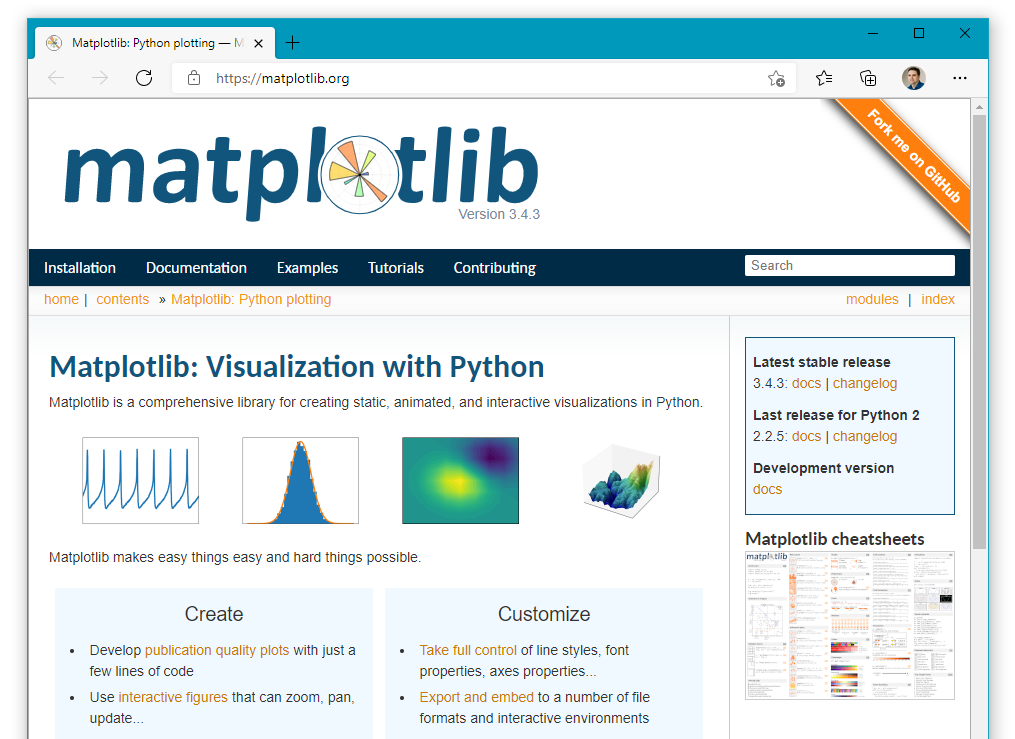
\includegraphics[scale=0.32]{image/matplotlib.png}} \\
\vspace{0.3cm}
\href{https://matplotlib.org/}{\beamerbutton{Открыть}}
\end{frame}

\subsection{Установка библиотеки}
\begin{frame}{Библиотека matplotlib}
\textbf{\# Установка библиотеки matplotlib} \\
\vspace{0.5cm}
pip install matplotlib
\end{frame}

\subsection{Вывод графика}
\begin{frame}{Вывод графика}
\lstinputlisting[language=Python]{code_04/41.py}
\vspace{0cm}
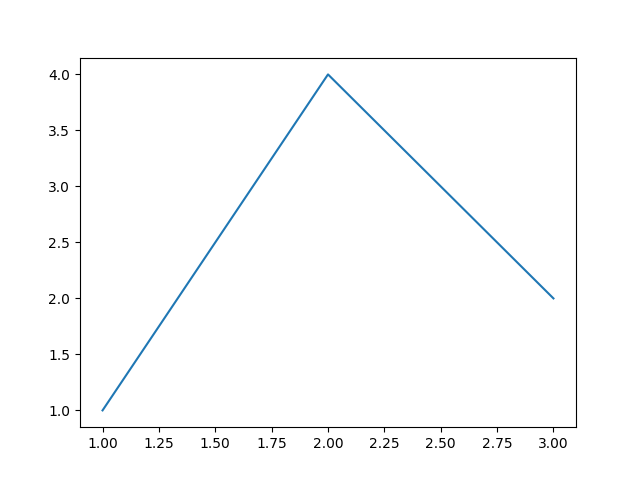
\includegraphics[scale=0.35]{code_04/41.png}
\end{frame}


\begin{frame}{Заголовок, подписи, легенда}
\lstinputlisting[language=Python]{code_04/42_1.py}
\vspace{0cm}
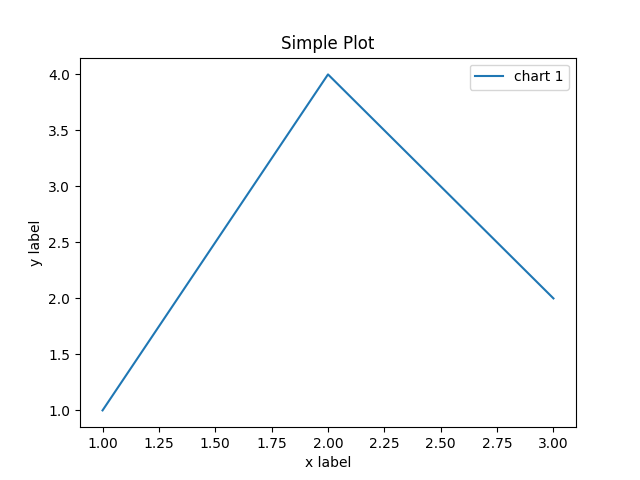
\includegraphics[scale=0.35]{code_04/42.png}
\end{frame}

\begin{frame}{Два и более графиков}
\lstinputlisting[language=Python]{code_04/43_1.py}
\vspace{0cm}
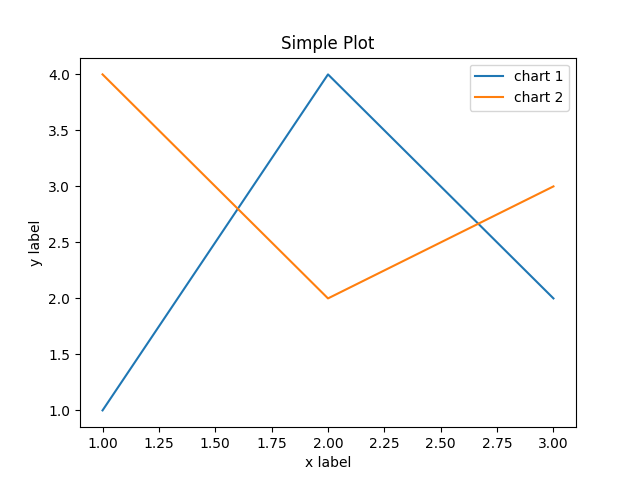
\includegraphics[scale=0.35]{code_04/43.png}
\end{frame}

\begin{frame}{Сетка}
\lstinputlisting[language=Python]{code_04/44_1.py}
\vspace{0cm}
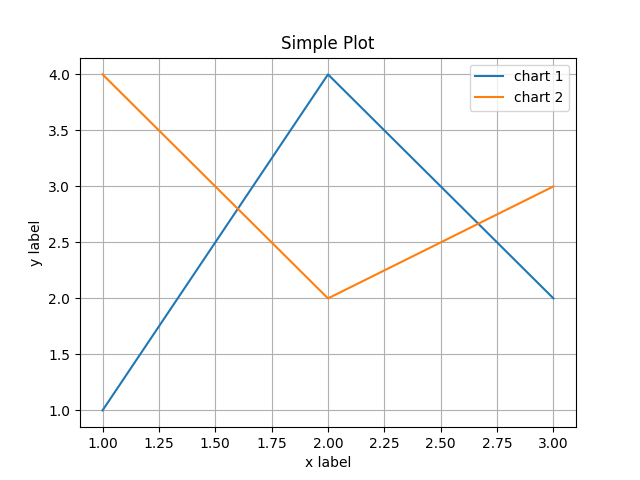
\includegraphics[scale=0.35]{code_04/44.png}
\end{frame}


\section{Математическая библиотека numpy}
\begin{frame}[t]{Оглавление}
\tableofcontents[currentsection]
\end{frame}

\subsection{Установка библиотеки}
\begin{frame}{Библиотека numpy}
\textbf{\# Установка библиотеки numpy} \\
\vspace{0.5cm}
pip install numpy \\
\vspace{0.2cm}
pip install scipy
\end{frame}


\begin{frame}{График функции y = sin(x)}
\lstinputlisting[language=Python]{code_04/45.py}
\end{frame}


\part{2}
\begin{frame}[t]{Вопросы}
\vspace{0.7cm}
\center{
\includegraphics[scale=0.3]{image/questions.jpg}} \\
\end{frame}

\end{document}